\documentclass[11pt,a4paper]{article}
\usepackage[spanish,es-nodecimaldot]{babel}	% Utilizar español
\usepackage[utf8]{inputenc}					% Caracteres UTF-8
\usepackage{graphicx}						% Imagenes
\usepackage[hidelinks]{hyperref}			% Poner enlaces sin marcarlos en rojo
\usepackage{fancyhdr}						% Modificar encabezados y pies de pagina
\usepackage{float}							% Insertar figuras
\usepackage[textwidth=390pt]{geometry}		% Anchura de la pagina
\usepackage[nottoc]{tocbibind}				% Referencias (no incluir num pagina indice en Indice)
\usepackage{enumitem}						% Permitir enumerate con distintos simbolos
\usepackage[T1]{fontenc}					% Usar textsc en sections
\usepackage{amsmath}						% Símbolos matemáticos
\usepackage{multirow}

\usepackage{listings}
\usepackage[dvipsnames]{xcolor}

\definecolor{codegreen}{rgb}{0,0.6,0}
\definecolor{codegray}{rgb}{0.5,0.5,0.5}
\definecolor{codepurple}{rgb}{0.58,0,0.82}
\definecolor{backcolour}{rgb}{0.95,0.95,0.92}

\lstdefinestyle{mystyle}{
    backgroundcolor=\color{backcolour},   
    commentstyle=\color{codegreen},
    keywordstyle=\color{magenta},
    numberstyle=\tiny\color{codegray},
    stringstyle=\color{codepurple},
    basicstyle=\ttfamily\footnotesize,
    breakatwhitespace=false,         
    breaklines=true,                 
    captionpos=b,                    
    keepspaces=true,                 
    numbers=left,                    
    numbersep=5pt,                  
    showspaces=false,                
    showstringspaces=false,
    showtabs=false,                  
    tabsize=4,
    language=C++
}

\lstset{style=mystyle}

% Comando para poner el nombre de la asignatura
\newcommand{\asignatura}{Arquitectura y Computación de Altas Prestaciones}
\newcommand{\autor}{Vladislav Nikolov Vasilev}
\newcommand{\titulo}{Práctica 5}
\newcommand{\subtitulo}{Paralelización del filtro de mediana mediante CUDA}
\newcommand{\rama}{Ingeniería de Computadores}

% Configuracion de encabezados y pies de pagina
\pagestyle{fancy}
\lhead{\autor{}}
\rhead{\asignatura{}}
\lfoot{Grado en Ingeniería Informática}
\cfoot{}
\rfoot{\thepage}
\renewcommand{\headrulewidth}{0.4pt}		% Linea cabeza de pagina
\renewcommand{\footrulewidth}{0.4pt}		% Linea pie de pagina

\begin{document}
\pagenumbering{gobble}

% Pagina de titulo
\begin{titlepage}

\begin{minipage}{\textwidth}

\centering

%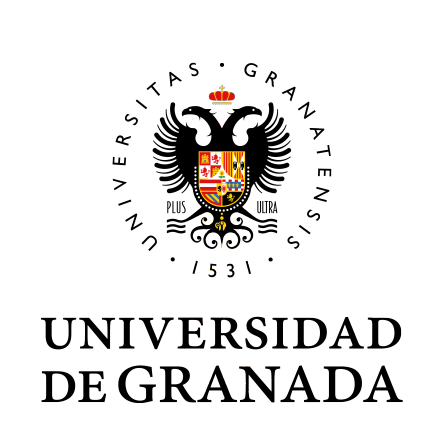
\includegraphics[scale=0.5]{img/ugr.png}\\

\includegraphics[scale=0.3]{img/logo_ugr.jpg}\\[1cm]

\textsc{\Large \asignatura{}\\[0.2cm]}
\textsc{GRADO EN INGENIERÍA INFORMÁTICA}\\[1cm]

\noindent\rule[-1ex]{\textwidth}{1pt}\\[1.5ex]
\textsc{{\Huge \titulo\\[0.5ex]}}
\textsc{{\Large \subtitulo\\}}
\noindent\rule[-1ex]{\textwidth}{2pt}\\[3.5ex]

\end{minipage}

%\vspace{0.5cm}
\vspace{0.7cm}

\begin{minipage}{\textwidth}

\centering

\textbf{Autor}\\ {\autor{}}\\[2.5ex]
\textbf{Rama}\\ {\rama}\\[2.5ex]
\vspace{0.3cm}


\includegraphics[scale=0.3]{img/etsiit.jpeg}

\vspace{0.7cm}
\textsc{Escuela Técnica Superior de Ingenierías Informática y de Telecomunicación}\\
\vspace{1cm}
\textsc{Curso 2019-2020}
\end{minipage}
\end{titlepage}

\pagenumbering{arabic}
\tableofcontents
\thispagestyle{empty}				% No usar estilo en la pagina de indice

\newpage

\setlength{\parskip}{1em}

\section{Introducción}

El objetivo de esta práctica es paralelizar, mediante \texttt{CUDA}, un algoritmo secuencial que
trabaje con estructuras de datos 2D tales como podrían ser matrices. Una vez que se ha
paralelizado, se tienen que tomar medidas de los tiempos y obtener la ganancia según la
cantidad de trabajo que tenga que hacer cada hebra (granularidad). Los tiempos
obtenidos se compararán con los de la versión secuencial y la versión en \texttt{MPI}, la cuál
fue implementada anteriormente. Este estudio se tiene que hacer con dos problemas de tamaño
diferente, uno más pequeño y uno más grande.

\section{Algoritmo escogido: filtro de mediana}

El algoritmo que se ha escogido paralelizar es el \textbf{filtro de mediana}. Este es un
filtro bastante sencillo y utilizado en el procesamiento de imágenes ya que permite eliminar
el \textbf{ruido sal y pimienta} de estas. Este tipo de ruido se caracteriza por la presencia
de píxeles blancos y negros en la toda la imagen, los cuáles son producto de alguna perturbación
de la señal de la imagen. Un ejemplo se puede ver a continuación:

\begin{figure}[H]
    \centering
    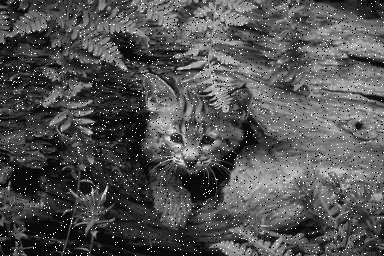
\includegraphics[scale=0.6]{img/cat.png}
    \caption{Imagen con ruido sal y pimienta.}
    \label{fig:cat}
\end{figure}

El algoritmo consiste en iterar sobre los píxeles de la imagen, coger una región de tamaño
$k \times k$ píxeles alrededor del actual (donde $k$ es el tamaño del filtro), ordenar
los valores y escoger el valor mediano, el cuál será el píxel de salida. Un ejemplo de este
procedimiento se puede ver a continuación:

\begin{figure}[H]
  \centering
  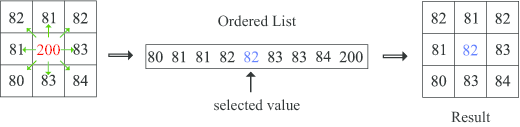
\includegraphics[scale=0.4]{img/median-filter.png}
  \caption{Ejemplo del filtro de mediana.}
  \label{fig:median-filter}
\end{figure}

Si aplicamos este filtro a la figura \ref{fig:cat}, obtendríamos el siguiente resultado:

\begin{figure}[H]
  \centering
  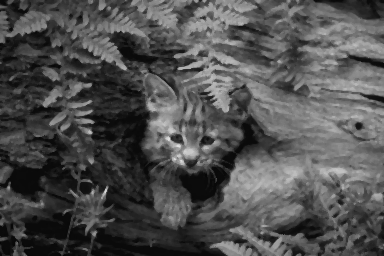
\includegraphics[scale=0.6]{img/filtered-cat}
  \caption{Imagen a la que se le ha aplicado el filtro de mediana.}
  \label{fig:filtered-cat}
\end{figure}

\section{Paralelización}

Ya que la versión secuencial fue explicada anteriormente, vamos a pasar a hablar directamente
de la paralelización que se ha realizado. En este caso, la paralelización es diferente a la que
se hacía en \texttt{MPI}, ya que siguen filosofías diferentes.

Se parte de una imagen de tamaño $w \times h$, donde $w$ es la anchura y $h$ la altura. La
imagen de salida tiene el mismo tamaño, pero recordemos que para poder aplicar el filtro se
tienen que replicar los bordes la imagen. Esto se hace para que el filtro se pueda aplicar de
igual manera por toda la imagen original, incluso por los bordes, donde en un principio, si
no se replicasen los bordes, se tendrían menos píxels, lo cuál obligaría a hacer un filtro
adaptativo al entorno del píxel. Esto sería contraproducente, ya que implicaría introducir
bloques condicionales en el \textit{kernel}, y al ejecutar todas las hebras el mismo código,
se ejecutaría dicho bloque de manera casi secuencial.

Esta replicación se hace al cargar la imagen, con lo cuál el \textit{kernel} no se tiene que
preocupar por eso. Recordemos que al replicar los bordes, la imagen sobre la que se aplica el
filtro es algo como lo que se puede ver a continuación:

\begin{figure}[H]
  \centering
  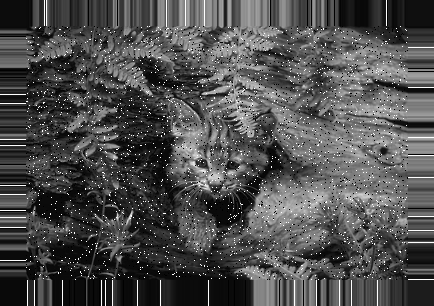
\includegraphics[scale=0.6]{img/borders-cat}
  \caption{Ejemplo de la replicación de bordes con filtro de tamaño $k = 101$.}
  \label{fig:borders-cat}
\end{figure}

Ya que estamos trabajando con una estructura de datos 2D como es una imagen, lo lógico es
crear un \textit{grid} 2D donde cada bloque esté indexado por una pareja $(x, y)$, donde $x$
es el índice en la dimensión $X$ e $y$ el índice en la dimensión $Y$. Cada bloque se
encargará de generar una región de $n \times n$ píxeles de la imagen de salida.
Se tiene por tanto que el \textit{grid} tiene un tamaño de $\frac{w}{n} \times \frac{h}{n}$
bloques. Para asegurar un reparto correcto, lo mejor es trabajar con imágenes cuya anchura y
altura sean potencias de 2, además de que el valor de $n$ también tiene que ser una potencia
de 2. De esta forma, no habrá bloques que generen regiones que se salgan de los límites de la
imagen, por ejemplo.

Aparte de esto, se tiene que los bloques también son bidimensionales, de manera que cada región
de la imagen de salida es generada de forma más fácil. Esto significa que se tiene \textbf{un
\textit{grid} 2D de bloques 2D}.

En cada bloque, cada hebra estará identificada por una pareja $(x_t, y_t)$, donde $x_t$ es el
índice en la dimensión $X$ del bloque e $y_t$ es el índice en la dimensión $Y$ del bloque.
Cada hebra se encargará de procesar una región dentro del bloque de $m \times m$ píxeles.
Cuanto menor sea el valor de $m$, se tendrá una granularidad más fina, mientras que a mayor
valor se tendrá una granularidad más gruesa, ya que cada hebra hará más trabajo. En un bloque
habrán $\frac{n}{m} \times \frac{n}{m}$ hebras, de manera que a menor valor, habrán más hebras,
mientras que a mayor valor, menos. Al ser $n$ una potencia de 2, para asegurar un reparto
correcto $m$ tendría que ser una potencia de 2 también, de manera que el reparto de trabajo
sea equitativo.

Para poder aplicar el filtro correctamente en cada bloque y generar una región de $n \times n$
píxeles hacen falta píxeles de los bloques vecinos, y de los bordes en el caso de que el bloque
esté en un extremo. Esto, por tanto, implica que cada bloque debe tener algo como una
\textbf{ventana local}, la cuál va a contener los píxels a utilizar. El tamaño de esta ventana
es de $l \times l$ píxeles, donde $l$ viene dado por:

\begin{equation}
l = n + 2 \cdot b
\end{equation}

\noindent donde $b$ es el tamaño del borde, el cuál es el resultado de la división entera
$\lfloor \frac{k}{2} \rfloor$.

Es de suma importancia destacar un aspecto muy importante, y es que, a pesar de que una
imagen se pueda representar como un \textit{array} 2D, tenemos que transformar dicho
\textit{array} a uno 1D. Esto se debe a que las funciones de reserva de memoria de
\texttt{CUDA} reservan memoria en posiciones contiguas, y es mucho más fácil hacer esto para
\textit{arrays} 1D que para los 2D. Por tanto, en vez de tener una estructura 2D con $h$ filas
y $w$ columnas, tendremos un \textit{array} 1D de tamaño $h \times w$. De la posición $0$ a
la $w-1$ irá la primera fila, de la $w$ a la $2w - 1$ la segunda, y así consecutivamente hasta
llegar a la última fila, la cuál irá desde la posición $(h-1)w$ hasta la $hw - 1$.

Una vez que hemos hablado de cómo se hace la división de la imagen en bloques y hebras y de
cómo se representan las imágenes, vamos a ver cómo se ha implementado el \textit{kernel} y lo
vamos a ir comentando. Dicho \textit{kernel} puede encontrarse en el fichero
\texttt{medianKernel.cu}, y a continuación se muestra dicho código:

\begin{lstlisting}
__global__ void medianKernel(float* dSrc, float* dDest,
							 int srcWidth, int destWidth,
							 int kernelSize, int windowSize,
							 int expandedWindowSize,
							 int pixelsPerThread)
{
    // Window which contains all the pixels that will be used in this block
    extern __shared__ float localWindow[];

    int xStartBlock = blockIdx.x * windowSize;
    int yStartBlock = blockIdx.y * windowSize;

    int xIdx = threadIdx.x;
    int yIdx = threadIdx.y;

    int xStartWindow = xIdx * pixelsPerThread;
    int yStartWindow = yIdx * pixelsPerThread;

    // Load local window from global memory and store it in local memory
    for (int j = yIdx; j < expandedWindowSize; j += blockDim.y)
    {
        for (int i = xIdx; i < expandedWindowSize; i += blockDim.x)
        {
            localWindow[j*expandedWindowSize + i] = dSrc[
            (yStartBlock + j) * srcWidth + xStartBlock + i];

        }
    }

    // Wait for all threads in the block to finish loading the data
    __syncthreads();

    // Allocate memory for kernel
    int kernelSquareSize = kernelSize * kernelSize;
    float* kernel = new float[kernelSquareSize];

    // Process local region inside local window
    for (int j = 0; j < pixelsPerThread; j++)
    {
        for (int i = 0; i < pixelsPerThread; i++)
        {
            // Get kernel's values
            for (int y = 0; y < kernelSize; y++)
            {
                for (int x = 0; x < kernelSize; x++)
                {
                    kernel[y*kernelSize + x] =
                    localWindow[(yStartWindow + j + y) * 
                       expandedWindowSize + xStartWindow + i + x];
                }
            }

            // Sort values and get median
            thrust::sort(thrust::seq, kernel,
            	kernel + kernelSquareSize);
            float median = kernel[kernelSquareSize / 2];
            dDest[(yStartBlock + yStartWindow + j) * destWidth +
            	xStartBlock + xStartWindow + i] = median;
        }
    }

    // Free memory
    delete[] kernel;
}
\end{lstlisting}

En la línea 8 se declara un \textit{array} dinámico compartido por todas las hebras de
un bloque. Esta es la manera de declararlo, y más adelante veremos cómo se hace la reserva
de memoria, la cuál se hace antes de la llamada al \textit{kernel}. Este \textit{array}
contendrá la \textbf{ventana local} de la que se habló anteriormente, es decir, todos los píxeles
que se van a necesitar para producir la región de salida. Al tener dicha información
en memoria local, los accesos posteriores van a ser más rápidos que si se quisiera acceder
a memoria global.

Una vez hecho esto se obtienen las posiciones de inicio del bloque (líneas 10-11). Se
multiplican los índices por el \textit{tamaño de ventana} o tamaño de bloque (a lo que
anteriormente habíamos llamado $n$). Los valores obtenidos hacen referencia son coordenadas
2D, pero más adelante se harán las transformaciones necesarias para que el acceso sea al
\textit{array} 1D. Se obtienen también los índices de las hebras y los índices de inicio en
la ventana/bloque (líneas 16-17). Estos últimos índices dependen de la granularidad (variable
\texttt{pixelsPerThread}).

Una vez hecho esto, en las líneas 20-28 se puede ver un doble bulce anidado. Su funcionalidad
es acceder a memoria global y copiar los píxeles necesarios para rellenar la
\textbf{ventana local}. El trabajo se reparte entre todas las hebras del bloque, de manera
que todas participen a la hora de traer los datos.

Una vez que la hebra ha terminado de copiar los datos que le correspondían tiene que esperar a
que todas terminen, ya que antes de continuar la \textbf{ventana local} tiene que tener
todos los datos. Esto se debe a que puede que haya alguna hebra que todavía no haya terminado
de copiar su parte y que otra hebra necesite acceder a esa información, con lo cuál se produciría
un error, ya que la información no está disponible todavía. Para ello, en la línea 31 se ha
introducido una llamada a una función de sincronización. De esta manera, hasta que todas las
hebras no hayan ejecutado esa función, no se podrá continuar con la ejecución del
\textit{kernel}.

En las líneas 34-35 se declara el \textit{kernel}, el cuál es un \textit{array} dinámico
1D local a cada hebra. Es en este \textit{array} donde se irán poniendo los valores del filtro
para posteriormente ordenarlos y obtener la mediana, el cuál será el píxel de salida.

En las líneas 38-60 se pueden ver cuatro bucles anidados. Los dos primeros bucles están
asociados a la granularidad. Es decir, hacen referencia a la región de tamaño $m \times m$ que
tiene que rellenar cada hebra dentro de la ventana/bloque, tal y como comentamos antes.
Los dos bulces internos (líneas 43-51) son los encargados de rellenar el \textit{kernel}
a partir de la \textbf{ventana local} para un píxel dado. Una vez que el \textit{kernel} está
relleno, se le aplica un algoritmo de ordenación (llamada a la función \texttt{thrust::sort()}).
Esta función ya está implementada dentro de las bibliotecas \texttt{CUDA}, y para que
pueda ser ejecutada por una hebra debe indicarse que la política (primer parámetro)
es secuencial mediante el valor \texttt{thrust::seq}. Una vez que el \textit{kernel} está
ordenado, se obtiene la mediana y posteriormente se asigna al correspondiente píxel de salida.

Finalmente, pero no por ello menos importante, una vez que la hebra ha terminado de procesar
su región $m \times m$ se tiene que liberar la memoria reservada para el \textit{kernel}
(línea 63).

Para poder exponer el \textit{kernel} al programa principal se ha creado un \textit{wrapper}
mediante una función normal de \texttt{C++}. Se ha hecho así para evitar problemas a la hora
de compilar el código. Esta función se puede ver a continuación:

\begin{lstlisting}
float* medianFilter(float* hSrc, int width, int height,
					int kernelSize, int windowSize,
					int pixelsPerThread, double& execTime)
{
    // Size of image with replicated borders
    int borderSize = kernelSize / 2;
    int srcWidth = width + 2*borderSize;
    int srcHeight = height + 2*borderSize;

    // Allocate local memory for filtered image
    float* hDest = new float[width * height];

    // Allocate memory for images in devide
    float* dSrc;
    float* dDest;

    cudaMalloc(&dSrc, srcWidth * srcHeight * sizeof(float));
    cudaMalloc(&dDest, width * height  * sizeof(float));

    // Define grid and block sizes
    dim3 gridSize((width - 1) / windowSize + 1, (height - 1) / windowSize + 1, 1);
    dim3 blockSize(windowSize / pixelsPerThread, windowSize / pixelsPerThread, 1);

    // Compute size of shared memory (in Bytes)
    int expandedWindowSize = windowSize + borderSize * 2;
    int sharedMemory = expandedWindowSize * expandedWindowSize * sizeof(float);

    auto t1 = std::chrono::high_resolution_clock::now();

    // Copy image to device
    cudaMemcpy(dSrc, hSrc, srcWidth * srcHeight * sizeof(float),
    	cudaMemcpyHostToDevice);


    // Apply median filter by calling the kernel
    medianKernel<<<gridSize, blockSize, sharedMemory>>>(dSrc,
    	dDest, srcWidth, width, kernelSize, windowSize, 
    	expandedWindowSize, pixelsPerThread);

    // Copy result from device
    cudaMemcpy(hDest, dDest, width * height * sizeof(float),
    	cudaMemcpyDeviceToHost);


    auto t2 = std::chrono::high_resolution_clock::now();
    execTime = std::chrono::duration<double>(t2 - t1).count();

    // Free device memory
    cudaFree(dSrc);
    cudaFree(dDest);

    return hDest;
}
\end{lstlisting}

Lo primero que hace es calcular el tamaño del borde (a lo que llamamos $b$ anteriormente)
en la línea 6. En las líneas 7-8 se determina la anchura y altura de la imagen fuente (aquella
imagen que tiene los bordes replicados). Después, en la línea 11 se reserva memoria para la
imagen resultado en el \textit{host}. En las líneas 14-18 se declaran los \textit{arrays} que
estarán en el dispositivo y se reserva la memoria para ellos. En la línea 21 se declara
el tamaño del \textit{grid}, el cuál puede verse que será 2D. Posteriormente, en la línea
22 se declara el tamaño del bloque. Una vez hecho esto, en la línea 25 se calcula el tamaño
de la \textbf{ventana local} y en la 26 se calcula el tamaño de dicha ventana en bytes (se
reservará tanta memoria posteriormente). Se procede luego a copiar la imagen fuente al
dispositivo (líneas 31-32) y se llama al \textit{kernel} (líneas 36-38). Vemos que a la hora
de llamar al \textit{kernel}, además de especificar el tamaño del \textit{grid} y del 
\textit{bloque}, se especifica también cuánta memoria dinámica compartida se quiere reservar
para cada bloque. Esa memoria dinámica será la que se utilice para la \textbf{ventana local}.
Finalmente, en las líneas 41-42 se copia el resultado del dispositivo al \textit{host}.
Posteriormente se toman las medidas de tiempo y se libera la memoria reservada en el
dispositivo (líneas 49-50), y se retorna el resultado.


\section{Experimentación}

Una vez que hemos visto cómo se ha paralelizado el filtro de mediana, vamos a proceder a
hacer la experimentación. Antes de nada, vamos a medir el tiempo que tarda la versión secuencial
del programa y la versión en \texttt{MPI} con las mismas configuraciones que en la práctica 3
(1, 2 y 4 procesos). Estos se hace debido a que estamos en una arquitectura completamenete
diferente a la que teníamos en dicha práctica, con lo cuál hay que tomar de nuevo dichas
medidas. No obstante, solo se analizarán las de \texttt{CUDA}. La versión secuencial y la
versión de \texttt{MPI} estarán compiladas con optimización. Se ha intentado añadir optimización
a la versión de \texttt{CUDA}, pero la diferencia es apenas significativa, e incluso en algunos
casos empeora. Por tanto, no se va a optimizar dicha versión.

Para esta nueva versión del programa se medirá la ejecución de cada configuración 3 veces y
nos quedaremos con el tiempo de ejecución más favorable. En este caso, tenemos que probar tres
cargas de trabajo distintas. Por tanto, probaremos con regiones de $1 \times 1$, $2 \times 2$ y
$4 \times 4$ por hebra. El tamaño de bloque será en todos los casos de $32 \times 32$, ya que es
el único que nos permite tener más de 32 hebras por bloque con todas las configuraciones, el cuál
es el tamaño de un \textit{warp}. De esta forma tendremos 1024, 256 y 64 hebras por bloque,
respectivamente. El tamaño del filtro de nuevo será de $7 \times 7$.

Tal y como hicimos anteriormente, se va a medir el tiempo que tarda en copiarse la imagen
a la memoria del dispositivo, el tiempo de ejecución del \textit{kernel} y el tiempo que tarda
en transferirse la imagen resultado del dispositivo al \textit{host}.

Con los tiempos medidos de la versión de \texttt{CUDA} haremos un pequeño estudio de la ganancia,
comparándolos claro está con la versión secuencial. Además, compararemos los tiempos de ejecución
de las tres versiones con los casos más favorables para ver cuál de ellas es la mejor en cada
caso.

\section{Resultados obtenidos}

Tal y como se comentó anteriormente, se han hecho 3 ejecuciones con cada configuración.
A continuación se ofrece una tabla con los resultados, destacando en negrita los mejores:

\begin{table}[H]
\centering
\begin{tabular}{|c|c|c|}
\hline
\textbf{\begin{tabular}[c]{@{}c@{}}Píxeles que calcula cada\\ hebra en cada dimensión\end{tabular}} & \textbf{\begin{tabular}[c]{@{}c@{}}Tiempo problema\\ pequeño (s)\end{tabular}} & \textbf{\begin{tabular}[c]{@{}c@{}}Tiempo problema\\ grande (s)\end{tabular}} \\ \hline
\multirow{3}{*}{1} & 0.787811 & 45.2461 \\ \cline{2-3} 
 & \textbf{0.708568} & \textbf{44.9549} \\ \cline{2-3} 
 & 0.726259 & 45.1012 \\ \hline
\multirow{3}{*}{2} & \textbf{0.296242} & \textbf{17.9155} \\ \cline{2-3} 
 & 0.298811 & 18.0785 \\ \cline{2-3} 
 & 0.305204 & 18.0178 \\ \hline
\multirow{3}{*}{4} & 0.288754 & \textbf{15.6332} \\ \cline{2-3} 
 & \textbf{0.250583} & 15.6645 \\ \cline{2-3} 
 & 0.256281 & 15.9279 \\ \hline
\end{tabular}
\caption{Tiempos obtenidos para las distintas configuraciones de granularidad para los dos problemas. En negrita los mejores tiempos.}
\label{tab:times}
\end{table}

Si observamos la tabla, podemos ver que para los dos problemas, a medida que aumenta la
granularidad, el tiempo de ejecución va disminuyendo. El cambio más drástico se produce
al pasar de que cada hebra procese 1 píxel por cada dimensión (es decir, de procesar regiones
$1 \times 1$) a procesar 2 píxeles por cada dimensión, o lo que viene siendo lo mismo, regiones
de $2 \times 2$. A groso modo, el tiempo de ejecución se reduce en aproxmadamente un 60\%, lo
cuál es un porcentaje muy considerable. Al pasar de de procesar 2 píxeles por cada dimensión a
4, el tiempo de ejecución también se reduce, aunque lo hace de forma mucho menos pronunciada.

Esta evolución puede verse más claramente en la siguiente gráfica:

\begin{figure}[H]
  \centering
  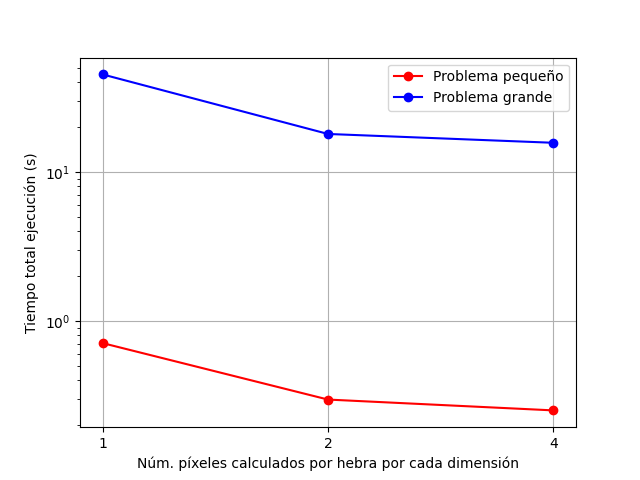
\includegraphics[scale=0.6]{img/speed}
  \caption{Evolución del tiempo de ejecución en función del número de píxeles que calcula
  cada hebra en cada una de las dimensiones de la imagen, en escala logarítmica.}
  \label{fig:time}
\end{figure}

Un posible motivo por el que el tiempo decrezca tanto al pasar de que cada hebra procese 1
píxel por cada dimensión a 2 es que esto provoca que haya una menor cantidad de hebras, pero
cada una de ellas hace más trabajo. O lo que es lo mismo, cada bloque de hebras produce una
salida del mismo tamaño, pero el trabajo que realiza cada hebra se ve incrementado. Esto, en
resumidas cuentas, significa un aumento de la granularidad.

En el primer caso, tenemos que para generar una región de la imagen de salida de $32 \times 32$
se necesitan 1024 hebras, mientras que en el segundo caso solo se necesitan 256 hebras. Esta
reducción del número de hebras implica bloques de hebras más pequeños, lo cuál a su vez implica
que haya que sincronizar una menor cantidad de hebras (recordemos que se debe esperar a que la
\textbf{ventana local} esté completamente cargada antes de continuar con la ejecución). Además,
al ser los bloques de hebras más pequeños, esto implica que estos tengan que esperar menos tiempo
para poder ser asignados a un procesador.

Al pasar de que cada hebra procese 2 píxeles por dimensión a 4, el tiempo de ejecución se ve
reducido en una menor medida, tal y como hemos comentado. Esto puede deberse a que la
granularidad empieza a ser demasiado grande para la cantidad de hebras que hay. En este caso
se tienen bloques de 64 hebras, y cada una de ellas genera una región de la imagen de salida
de $4 \times 4$ píxeles. Esto implica que, al ser los bloques más pequeños, tienen que esperar
menos a ser asignados a un procesador, pero este tiempo de espera posiblemente se vea afectado
por la cantidad de trabajo que tiene que hace cada hebra. Al tener que hacer más trabajo, más
tiempo se tardará en terminarlo.

Si aumentásemos la granularidad y tuviésemos que cada hebra calcula 8 píxeles por dimensión,
tendríamos bloques de 16 hebras en los que cada hebra calcula una región de $8 \times 8$. Esto
sería contraproducente, ya que estaríamos desaprovechando potencia de cómputo al ser los bloques
menores a lo que es un \textit{warp} de hebras, los cuáles son de 32 hebras, y además estaríamos
cargando demasiado cada hebra. Esto implica que, si seguimos aumentando la granularidad, llegará
en el momento en el que cada región de $32 \times 32$ se calcule secuencialemente, lo cuál
implica desaprovechar demasiado la capacidad de los procesadores de la \texttt{GPU}.

Una vez que hemos visto esto, vamos a hacer un pequeño estudio de la ganancia. Para obtener
la ganancia, vamos a tener como \textbf{tiempo base para el problema pequeño 0.520567 segundos},
mientras que para el \textbf{problema grande vamos a tener un tiempo base de 27.5843 segundos}.
A continuación se puede ver una tabla con la ganancia para cada configuración para las
distintas configuraciones, además de una gráfica que ilustra la evolución de la ganancia:

\begin{table}[H]
\centering
\begin{tabular}{|c|c|c|}
\hline
\textbf{\begin{tabular}[c]{@{}c@{}}Píxeles que calcula cada\\ hebra en cada dimensión\end{tabular}} & \textbf{\begin{tabular}[c]{@{}c@{}}Ganancia problema\\ pequeño\end{tabular}} & \textbf{\begin{tabular}[c]{@{}c@{}}Ganancia problema\\ grande\end{tabular}} \\ \hline
1 & 0.735 & 0.614 \\ \hline
2 & 1.757 & 1.54 \\ \hline
4 & 2.077 & 1.764 \\ \hline
\end{tabular}
\caption{Ganancia obtenidos para las distintas configuraciones de granularidad para los dos problemas.}
\label{tab:speedup}
\end{table}

\begin{figure}[H]
  \centering
  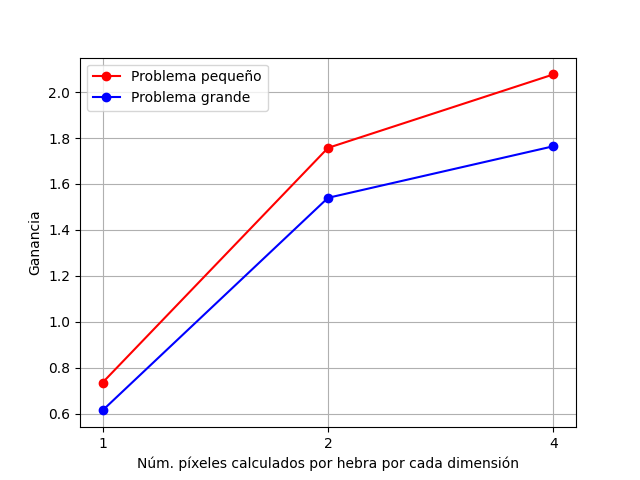
\includegraphics[scale=0.6]{img/speedup}
  \caption{Evolución de la ganancia en función del número de píxeles que calcula
  cada hebra en cada una de las dimensiones de la imagen.}
  \label{fig:speedup}
\end{figure}

Como podemos ver tanto en la tabla como en la gráfica, la ganancia empieza siendo baja y va
subiendo en los dos problemas. La ganancia crece más en el problema pequeño que en el grande,
pero crece de manera más o menos igual en ambos problemas. Vemos que en ambos casos la ganancia
crece mucho cuando se pasa de que cada hebra calcule 1 píxel pro dimensión a que calcule 2,
mientras que crece menos al pasar de 2 a 4. Esto es completamente normal, ya que como pudimos
ver en la figura \ref{fig:time}, el tiempo mejoró mucho menos al pasar de 2 a 4 píxeles por
dimensión.

Hay una serie de cosas que pueden llamar la atención. Por ejemplo, la ganancia para el caso
en el que cada hebra calcula 1 píxel por dimensión está por debajo de 1, ya que el tiempo de
ejecución de la versión de \texttt{CUDA} es inferior a la secuencial. Esto puede deberse
a que hay demasiadas hebras por bloque con una granularidad demasiado pequeña, lo cuál hace
que haya demasiados bloques inactivos en todo momento. Por tanto, para los dos problemas podríamos
decir que la asignación de carga de trabajo \textit{naive} no da buenos resultados.

Otra cosa que puede llamar la atención es que la ganancia obtenida en el problema grande es algo
menor que la del pequeño. Esto puede deberse a que, dentro del tiempo medido, se tiene en
cuenta también el tiempo de transferencia de los datos del \textit{host} al dispositivo
y del dispositivo al \textit{host}. Al tener el problema grande una imagen bastante grande,
estos tiempos son algo mayores, aunque tampoco demasiado, ya que el mayor parte del tiempo
se dedica al cómputo, ya que como es obvio, hay una mayor cantidad de bloques.

Por último, podemos ver que no obtenemos una ganancia demasiado grande en los dos problemas.
Como mucho, en el problema pequeño y con la mayor granularidad, obtenemos una ganancia de
aproximadamente 2. En el caso del problema grande dicha ganancia es aun menor, ya que 
no llega ni a $1.8$. Muy posiblemente, si seguimos aumentando la granularidad del problema
la ganancia crecerá o bien muy poco o bien empezará a decrecer debido a que se están
desaprovechando los recursos del \textit{dispositivo}. Por tanto, el límite de la ganancia
que tenemos en esta versión del programa es bastante pequeño, si lo comparamos con la
que por ejemplo obtuvimos en el caso de \texttt{MPI}.

Un posible motivo por el que los resultados no sean los esperados o lo suficientemente buenos
puede deberse a que la tarjeta gráfica no sea lo suficientemente potente. Si tuviésemos una
tarjeta más actual, los resultados posiblemente hubiesen sido muy diferentes, con unos
mejores tiempos y una mejor ganancia. Por tanto, las limitaciones técnicas de la \texttt{GPU}
han tenido su repercusión sobre los resultados. Recordemos que la tarjeta dispone de 5 SMs y
de 128 SPs por SM. Si la gráfica fuese algo más potente, el número de SMs sería mayor, lo cuál
implicaría poder ejecutar más bloques simultáneamente. Por tanto, estamos algo limitados
en este aspecto, y con \textit{hardware} más actual los resultados hubiesen sido bastante
distintos.

\section{Comparativa}

Una vez que hemos estudiado qué tal se comporta la versión de \texttt{CUDA} del programa,
vamos a comparar las tres versiones para ver cómo se comporta cada una de ellas en cada problema.
A continuación se ofrece una tabla con los casos más favorables para cada versión y cada problema,
acompañada de un gráfico de barras que agrupa los tiempos en función del problema:

\begin{table}[H]
\centering
\begin{tabular}{|c|c|c|}
\hline
\textbf{Versión del programa} & \textbf{\begin{tabular}[c]{@{}c@{}}Tiempo problema\\ pequeño (s)\end{tabular}} & \textbf{\begin{tabular}[c]{@{}c@{}}Tiempo problema\\ grande (s)\end{tabular}} \\ \hline
Secuencial & 0.520567 & 27.5843 \\ \hline
MPI & 0.316762 & 10.0926 \\ \hline
CUDA & 0.250583 & 15.6332 \\ \hline
\end{tabular}
\caption{Tiempos de ejecución más favorables para cada problema para las tres versiones del programa.}
\label{tab:times-versions}
\end{table}

\begin{figure}[H]
  \centering
  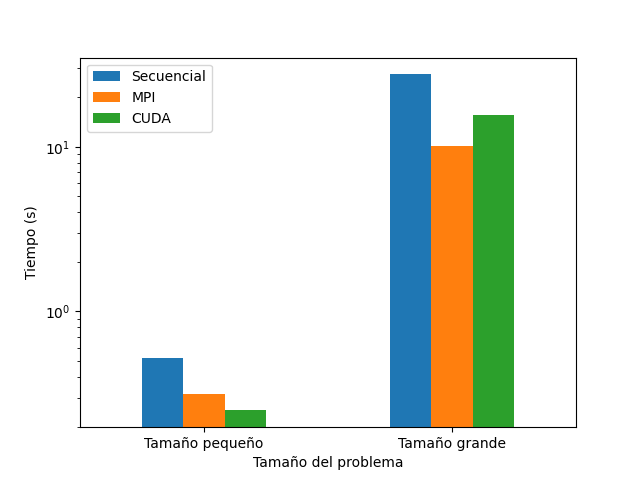
\includegraphics[scale=0.6]{img/comparison}
  \caption{Comparativa de los tiempos de ejecución para cada versión del programa en función
  del tamaño del problema, en escala logarítmica.}
\end{figure}

Como podemos ver, en los dos problemas la peor versión es la secuencial, ya que es la
que más tarda. La versión de \texttt{MPI} se queda un poco por detrás de la de \texttt{CUDA}
en el problema pequeño, mientras que en el problema grande es mejor que esta última.

El motivo por el que la versión de \texttt{CUDA} es más rápida que la de \texttt{MPI} en el
problema pequeño puede deberse a que, en esta última versión, se tarde bastante tiempo en
crear los procesos y asignar la carga de trabajo correspondiente en cada uno de ellos. Al
trabajar \texttt{CUDA} con hebras, el tiempo de creación de una hebra es mucho menor
que el de crear un proceso. Además, \texttt{CUDA} es más rápido en los tiempos de cómputo,
ya que permite ejecutar la misma instrucción para un montón de hebras
a la vez en vez de ejecutar el código de manera secuencial, que es lo que sucede con
\texttt{MPI} (aunque el código secuencial en un principio se ejecuta en distintos
cores/procesadores/nodos, dependiendo del equipo).

No obstante, para el problema grande, tal y como hemos dicho anteriormente, \texttt{MPI}
ofrece unos mejores tiempos que \texttt{CUDA}. El motivo por el que \texttt{CUDA} es más
lento en este caso puede deberse a que, para este problema, hay demasiados bloques de
hebras. A esto, si le sumamos las limitaciones del \textit{hardware} que comentamos
anteriormente, hace que haya muchos bloques que estén a la espera de ser asignados y ejecutados.
Por tanto, aunque el tiempo de inicialización de los procesos y de la distribución 
de la carga de trabajo sean superiores en \texttt{MPI}, y aunque el código de
\texttt{MPI} se ejecute secuencialmente, una vez que los procesos reciben su carga de
trabajo ya pueden empezar a trabajar sin esperar nada más, a diferencia de los bloques
de \texttt{CUDA}, los cuáles deben esperar a que se libere el procesador para poder
empezar a ser ejecutados.

No obstante, cabe destacar que \texttt{MPI} funciona muy bien en computación distribuida y
en problemas muy grandes, ya que permite aprovechar el cómputo de distintos equipos. Por tanto,
no es de extrañar que ofrezca buenos resultados en problemas grandes. También cabe destacar
que los resultados de \texttt{CUDA} en el caso del problema grande sean malos, sino todo lo
contrario. Posiblemente con una tarjeta más actual, los resultados hubiesen sido muy diferentes,
ya que estas al disponer de un mayor número de SMs, harían que los tiempos de ejecución fuesen
más bajos, ya que habría menos bloques esperando. Pero aun así, con todas las limitaciones,
\texttt{CUDA} ha demostrado ofrecer unos resultados aceptables incluso en problemas
grandes.

\section{Conclusiones}

En esta práctica hemos visto cómo se puede paralelizar el filtro de la mediana
en \texttt{CUDA} y cómo se puede hacer dicha paralelización de forma que las hebras
tengan una carga de trabajo variable.

Al hacer un estudio de los tiempos de ejecución y de la ganancia, nos hemos dado cuenta de
que es muy importante encontrar un equilibrio entre el tamaño de los bloques de hebras y la
cantidad de trabajo que tenga que realizar cada hebra del bloque. Tener bloques de hebras
demasiado grandes con poca carga de trabajo por hebra puede implicar que muchos de los bloques
estén esperando a ser asignados, mientras que tener bloques de hebras pequeños con mucha carga
de trabajo por hebra puede significar que se estén desaprovechando los recursos de la tarjeta.

También hemos visto que, en este caso, la ganancia obtenida estaba bastante limitada ganancia,
muy posiblemente por las limitaciones de la tarjeta que se ha utilizado, y que probablemente
con una tarjeta más actual o potente los resultados obtenidos podrían haber sido bastante mejores.

También hemos hecho una comparación de los mejores tiempos de ejecución de todas las versiones.
Ahí hemos visto que la versión secuencial, como era de esperarse, ha resultado ser la más lenta.
En cuando a las versiones de \texttt{CUDA} y \texttt{MPI}, hemos visto que la primera ha ofrecido
unos mejores resultados en el problema pequeño, mientras que la segunda lo ha hecho en el
problema grande. De aquí podemos extraer algunas conclusiones:

\begin{enumerate}
	\item Paralelizar siempre nos va a permitir mejorar los tiempos de ejecución, aunque
	hay que paralelizar ``con cabeza''. Es decir, no debemos hacer una paralelización excesiva
	ya que introducirá demasiados tiempos de \textit{overhead}, lo cuál al final hará que
	los tiempos empeoren.
	\item \texttt{MPI} y \texttt{CUDA} han demostrado ofrecer unos muy buenos resultados
	en ambos problemas, y son opciones muy interesantes que deben ser consideradas a la hora
	de paralelizar un algoritmo. Aunque, claro está, también depende del problema que nos
	enfrentemos, ya que en algunos casos una de las metodologías va a funcionar mejor que
	la otra.
\end{enumerate}

Por último, es importante destacar una cosa. A pesar de que \texttt{MPI} y \texttt{CUDA} ofrecen
filosofías diferentes, no son mútuamente excluyentes. Es más, podemos incluso combinarlas
para ofrecer unos mejores resultados. Por ejemplo, si tenemos un problema extremadamente
grande, podemos partirlo en problemas más pequeños y enviarlos a los distintos nodos de cómputos
de los que dispongamos. Dentro de esos nodos podemos utilizar las tarjetas gráficas para ejecutar
muy rápidamente el código. Una vez que se obtengan los resultados, se enviarían al nodo maestro
que ha hecho la división de trabajo. De esta manera, aprovecharíamos la facilidad que ofrece
\texttt{MPI} de distribuir el trabajo entre distintos nodos y luego de juntar los resultados con
la potencia de cómputo que ofrece \texttt{CUDA} al permitir ejecutar una misma instrucción
sobre múltiples datos.

Este es solo un ejemplo de cómo se podrían combinar dos filosofías diferentes para obtener
los mejores resultados. Ahora bien, cuando estemos ante un problema, debemos estudiar
qué filosofía se adapta mejor a éste, ya que no hay una solución universal que permita
resolver cualquier tipo de problema. Debemos, además de eso, tener en cuenta los recursos
de los que disponemos y cómo los podemos utilizar para resolver el problema al que
nos vayamos a enfrentar. Cada problema es un mundo, y por tanto, cada uno de ellos
puede ser resuelto de una manera diferente.

\end{document}

